
\begin{figure}[t]
    \centering

    % Row 1
    \begin{subfigure}[b]{0.45\linewidth}
        \centering
        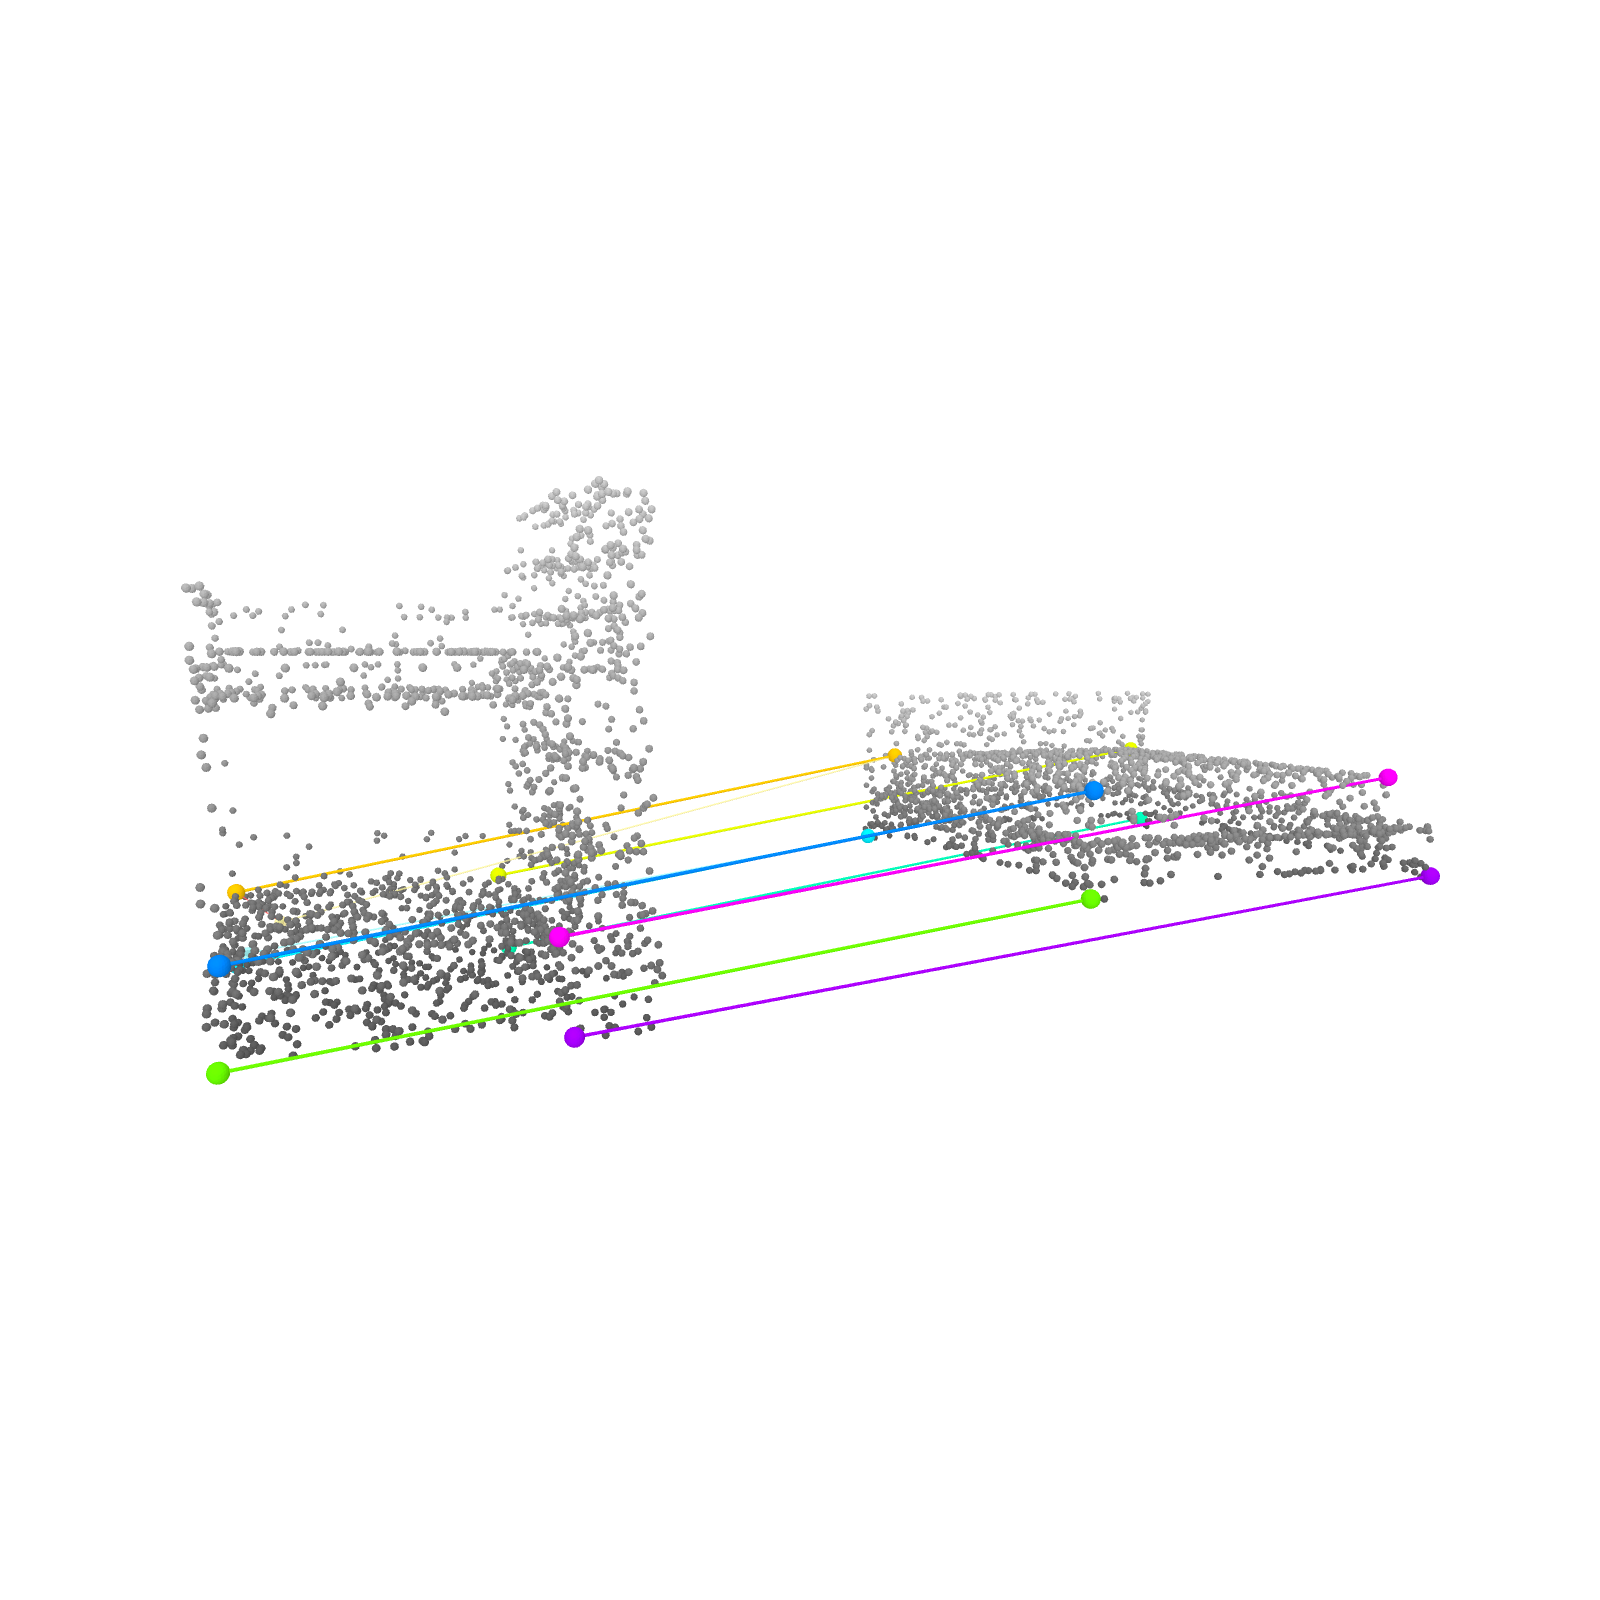
\includegraphics[trim={10 350 10 350},clip,width=\linewidth,height=\linewidth]{sup_mat/figures/bed_top11_ac97ffc6_x_e2532c6b_yaw-200p22_pitch84p01.png}
        \caption{Bed}
        \label{fig:square_bed}
    \end{subfigure}
    \hfill
    \begin{subfigure}[b]{0.45\linewidth}
        \centering
        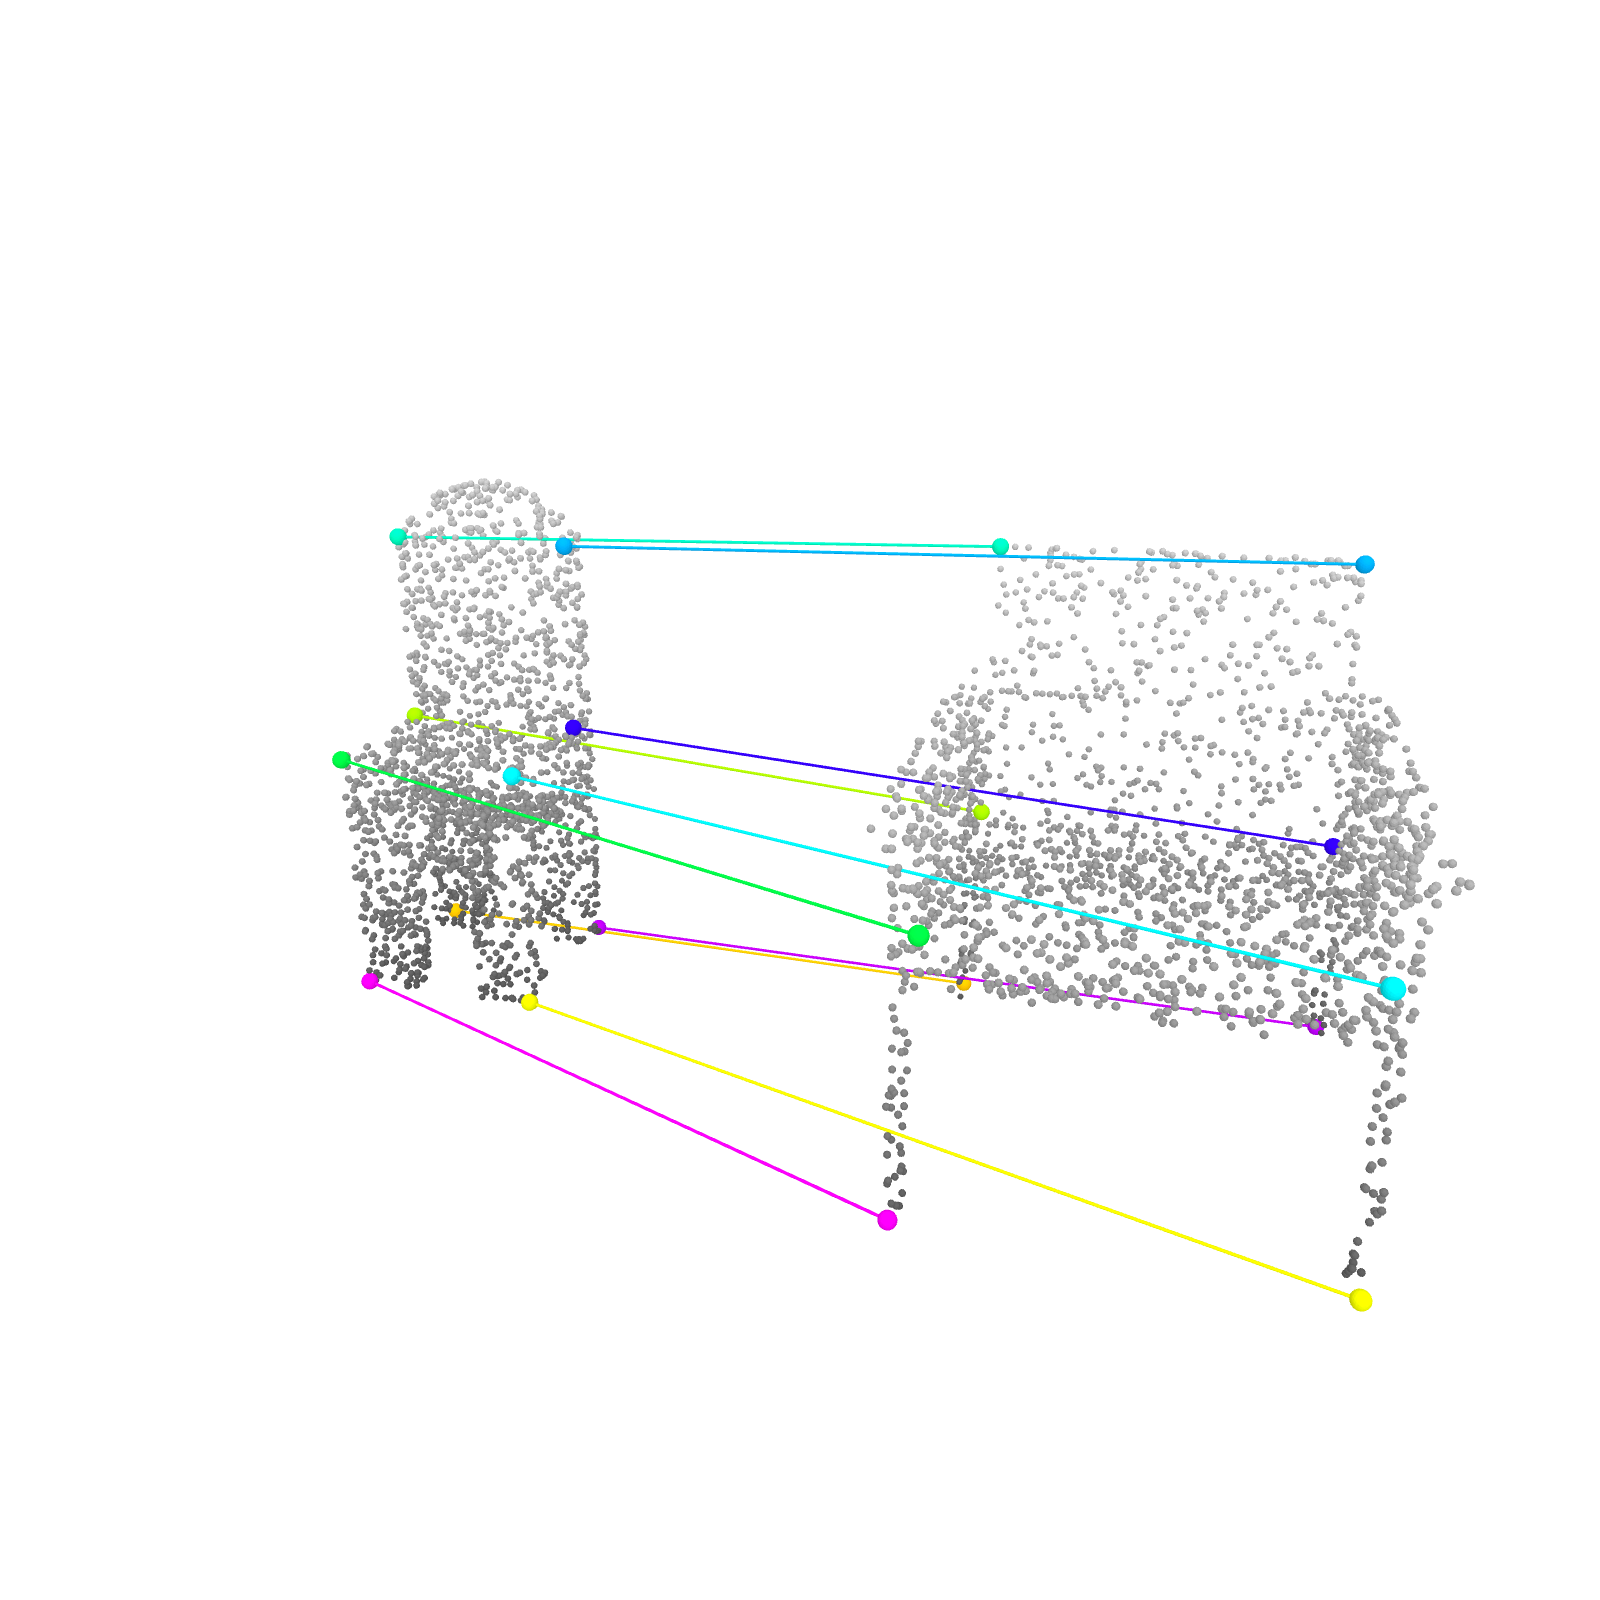
\includegraphics[trim={10 150 10 150},clip,width=\linewidth,height=\linewidth]{sup_mat/figures/chair_top11_2828b98d_x_4647b2b9_yaw-164p94_pitch69p52.png}
        \caption{Chair}
        \label{fig:square_chair}
    \end{subfigure}


    % Row 2
    \begin{subfigure}[b]{0.45\linewidth}
        \centering
        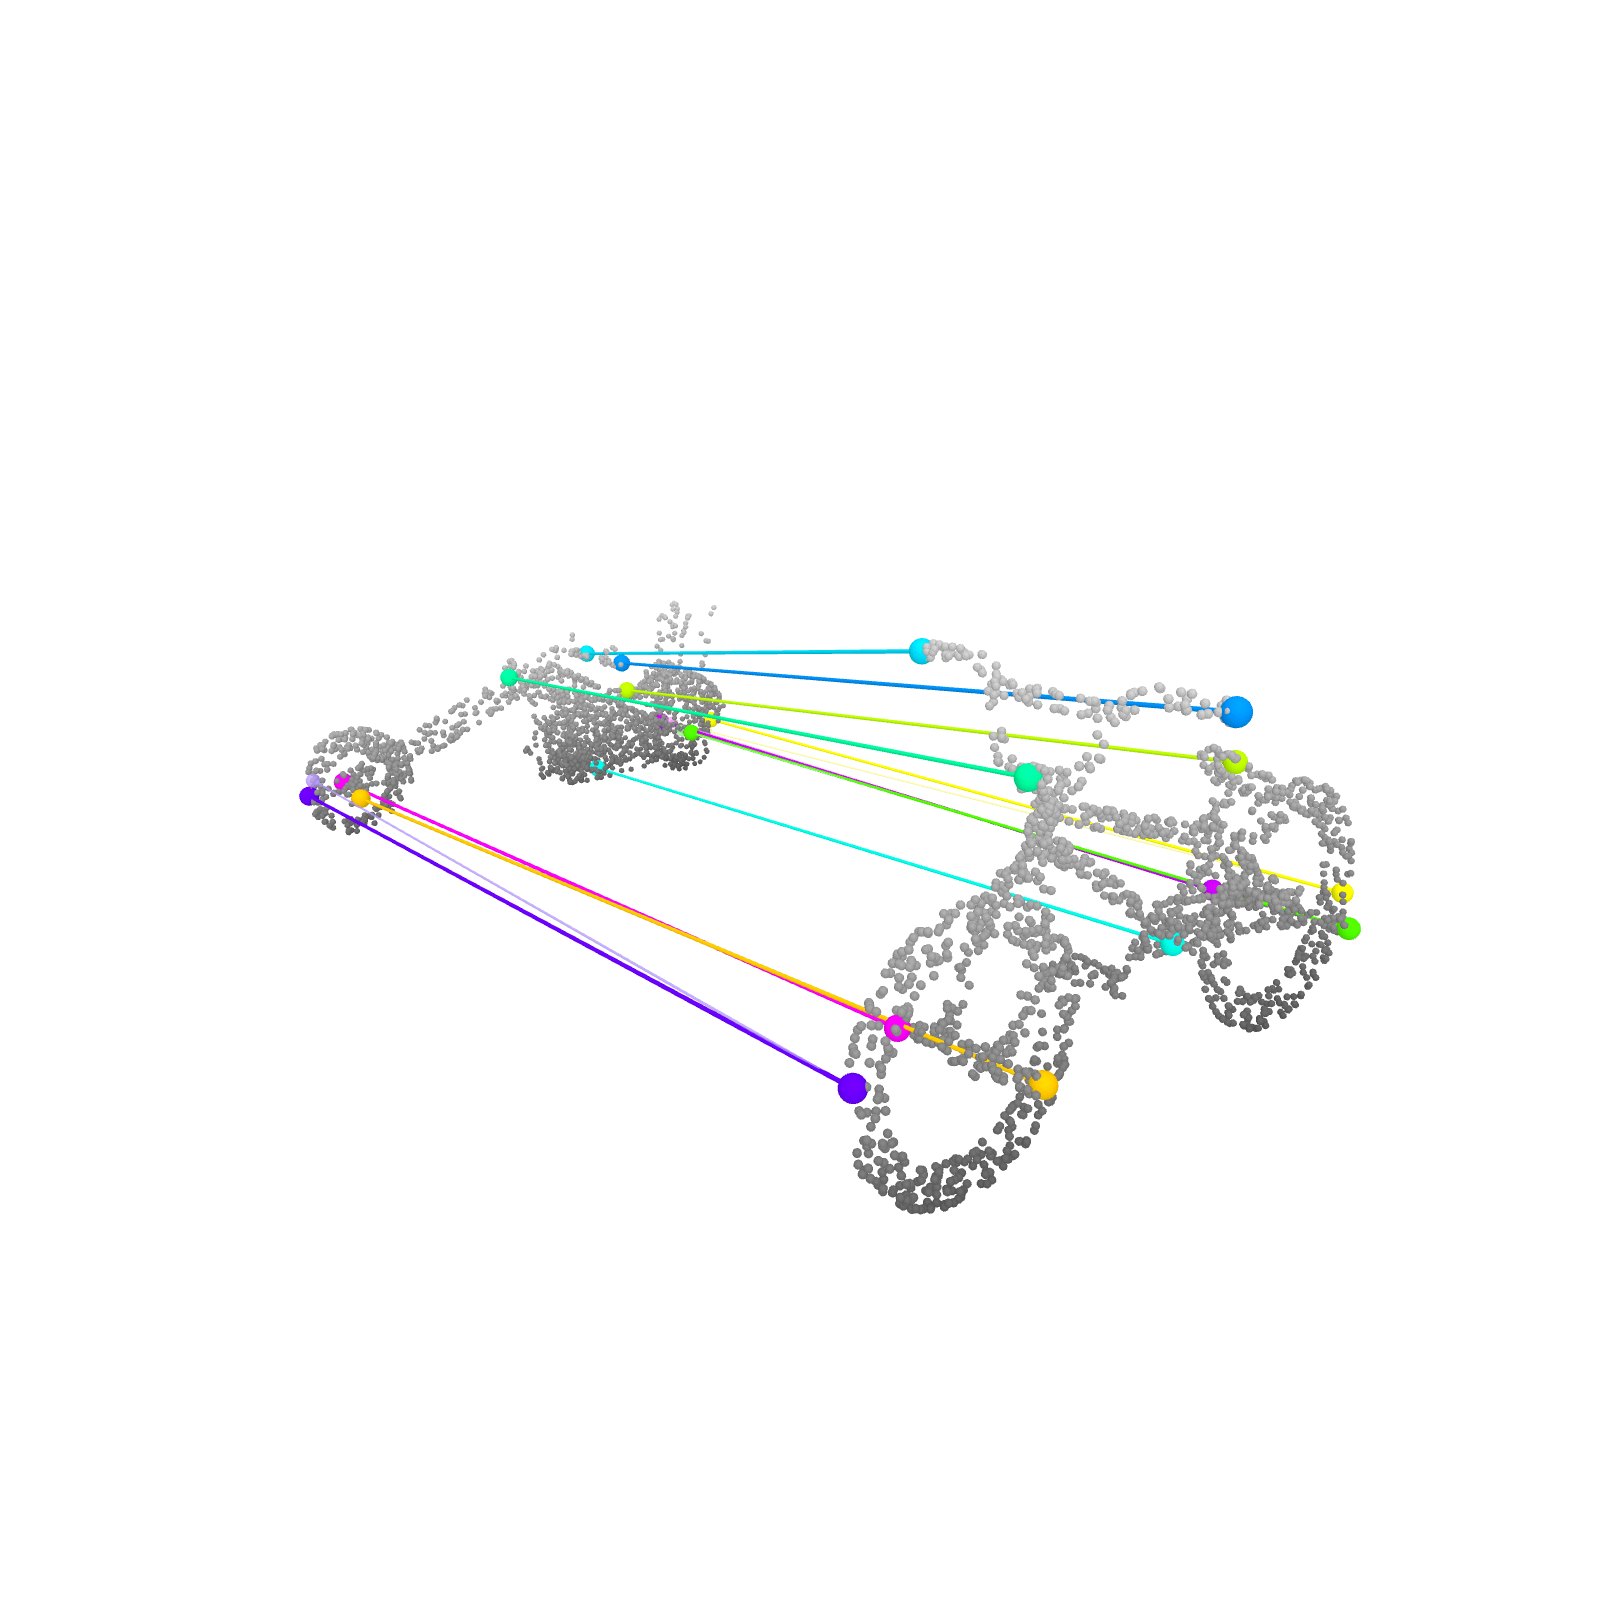
\includegraphics[trim={10 350 10 10},clip,width=\linewidth,height=\linewidth]{sup_mat/figures/motorcycle_top03_1d8fb258_x_a1553e0b_yaw-131p95_pitch72p26.png}
        \caption{Motorcycle}
        \label{fig:square_motorcycle}
    \end{subfigure}
    \hfill
    \begin{subfigure}[b]{0.45\linewidth}
        \centering
        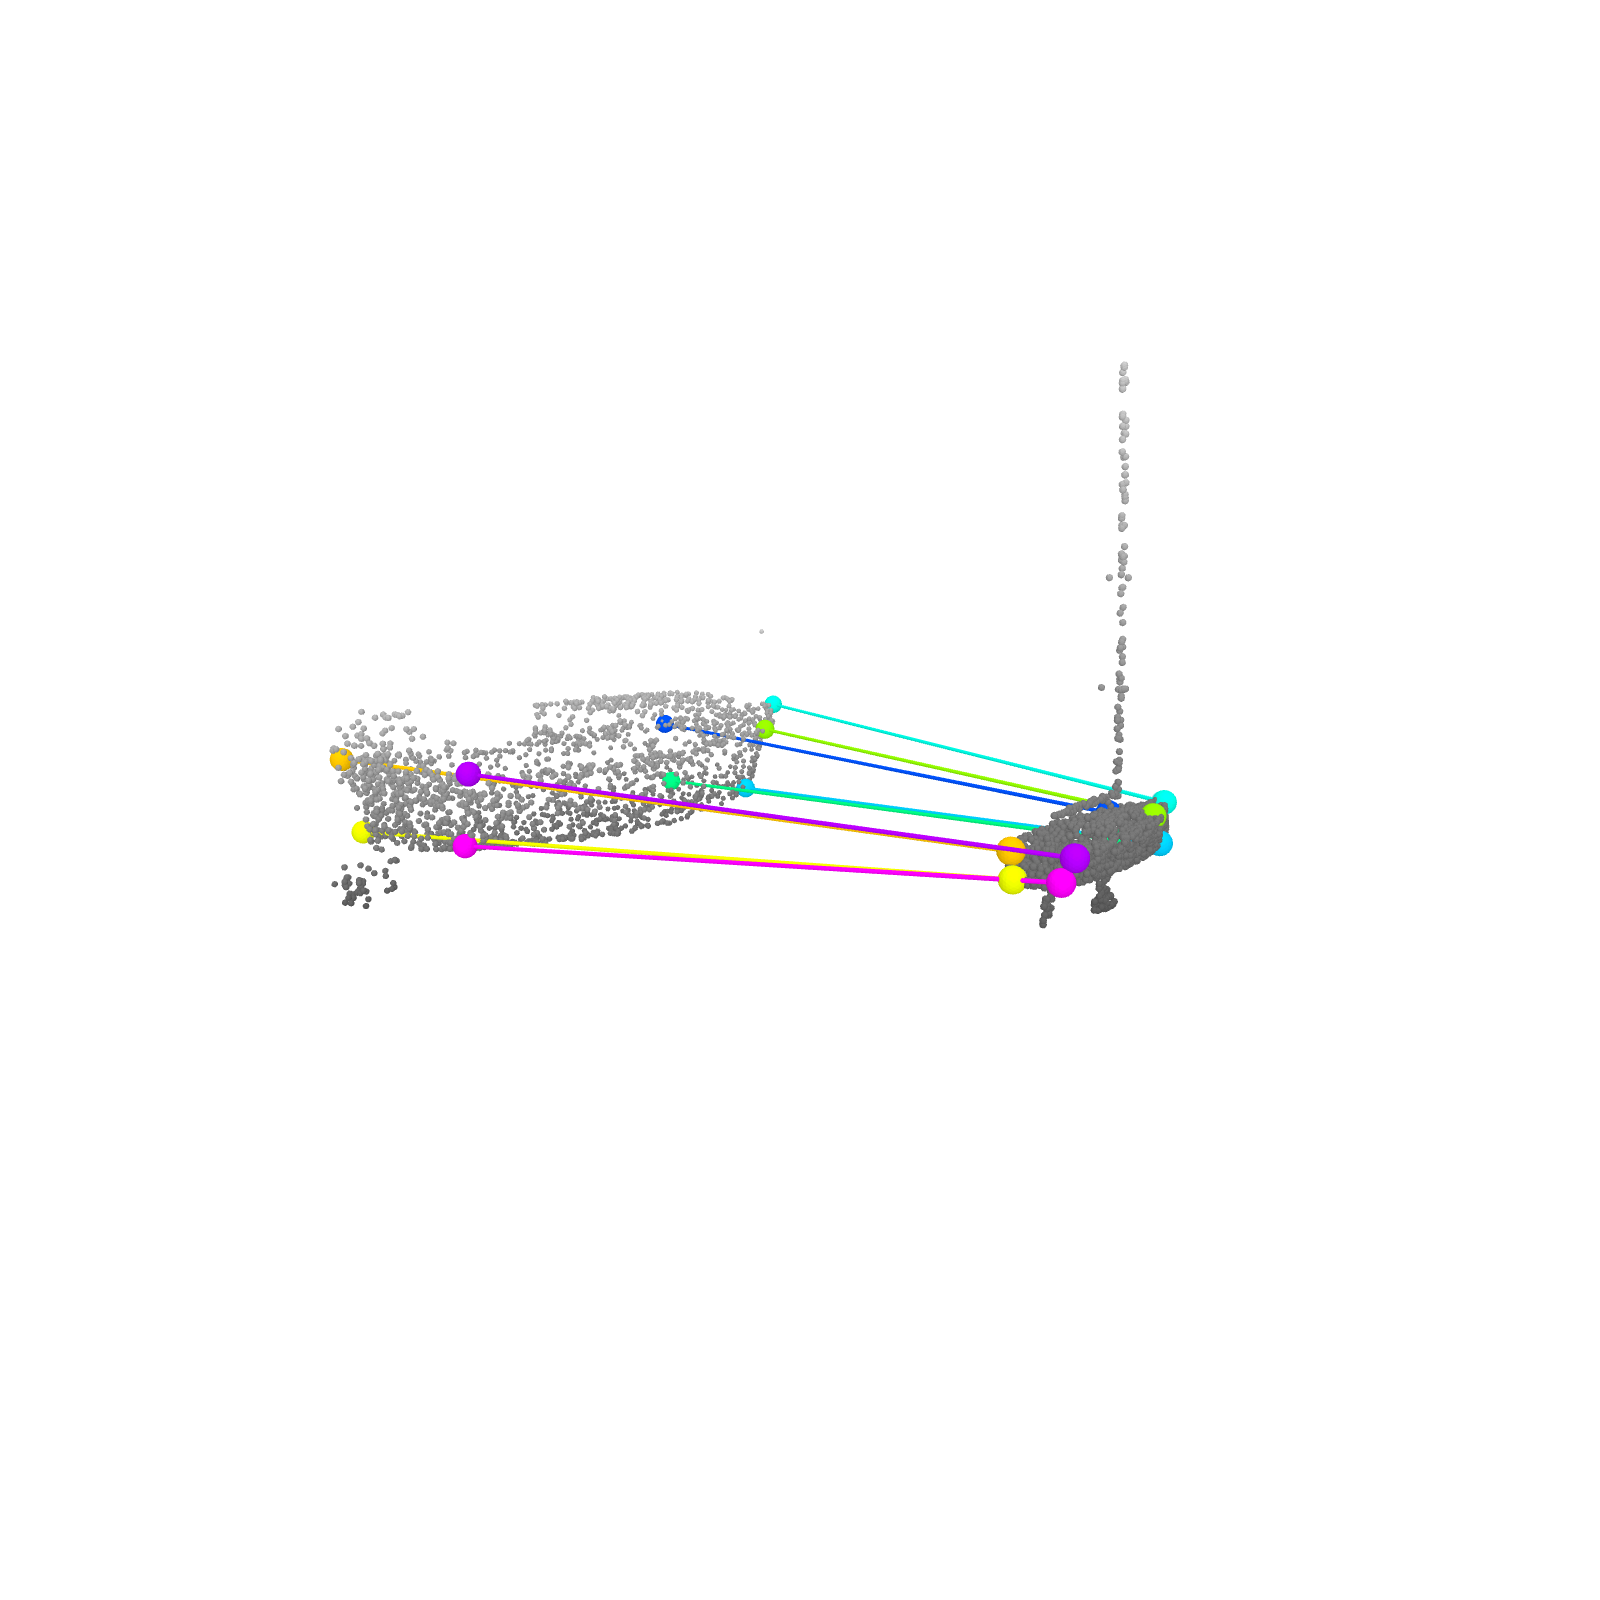
\includegraphics[trim={10 550 10 150},clip,width=\linewidth,height=\linewidth]{sup_mat/figures/vessel_top02_cc6656ba_x_e604463b_yaw-325p50_pitch80p49.png}
        \caption{Vessel}
        \label{fig:square_vessel}
    \end{subfigure}

    \caption{\textbf{Qualitative correspondence results on KeypointNet.} For each object pair, we use the human-annotated keypoints on the source object as queries and predict the corresponding points on the target object. Predicted correspondences are shown in lighter colors, while the human annotations are shown in darker colors. The close overlap between the two indicates that our pipeline recovers correspondences that are highly consistent with human semantic annotations.}
    \label{fig:four_square_images}
\end{figure}